\documentclass[final,hyperref={pdfpagelabels=false}]{beamer}
\mode<presentation>
{
  \usetheme{rc2018}
}
\usepackage[orientation=portrait,size=a0,scale=1.4,debug]{beamerposter}
\usepackage{siunitx}
%%%%%%%%%%%%%%%%%%%%%%%%%%%%%%%%%%%%%%%%%%%%%%%%%%%%%%%%%%%%%%%%%%%%%%%%%%%%%%%%% 5
\title{Influence of inhibitory circuits in the olfactory bulb on the frequency tuning of mitral cells}
\author[Miko]{Rebecca Miko, Christoph Metzner and Volker Steuber}
\institute{University of Hertfordshire, AL10 9AB, UK}
\date{Jul. 31th, 2018}

%%%%%%%%%%%%%%%%%%%%%%%%%%%%%%%%%%%%%%%%%%%%%%%%%%%%%%%%%%%%%%%%%%%%%%%%%%%%%%%%% 5
\begin{document}
\begin{frame}{} 
\begin{block}{Motivation}
The olfactory bulb (OB) in mammals is responsible for receiving, processing and relaying olfactory information (odours). 
Naturalistic odour stimuli have a rich temporal structure, caused by turbulent airflow that mixes the odorant with clean air and other odorants. 
Recent studies show that this structure contains information about the olfactory scene, for example the distance to an odour source $[1,2]$. 
Furthermore, it has been suggested that animals might exploit this structure and extract this information in order to find odour sources $[3]$. 
As some of this information may lie in the frequency content of the stimuli $[2]$, we studied input frequency dependent responses of mitral cells (MCs) in the olfactory bulb (OB), the first processing stage in the mammalian olfactory system.
Specifically, we investigated whether MCs show frequency tuning and, if they do, how different components of the glomerular layer circuitry shape and determine the tuning.
\end{block}
    
    
\begin{columns}[t]
\begin{column}{.48\linewidth}
    
\begin{block}{Model} 
\begin{figure}
\center
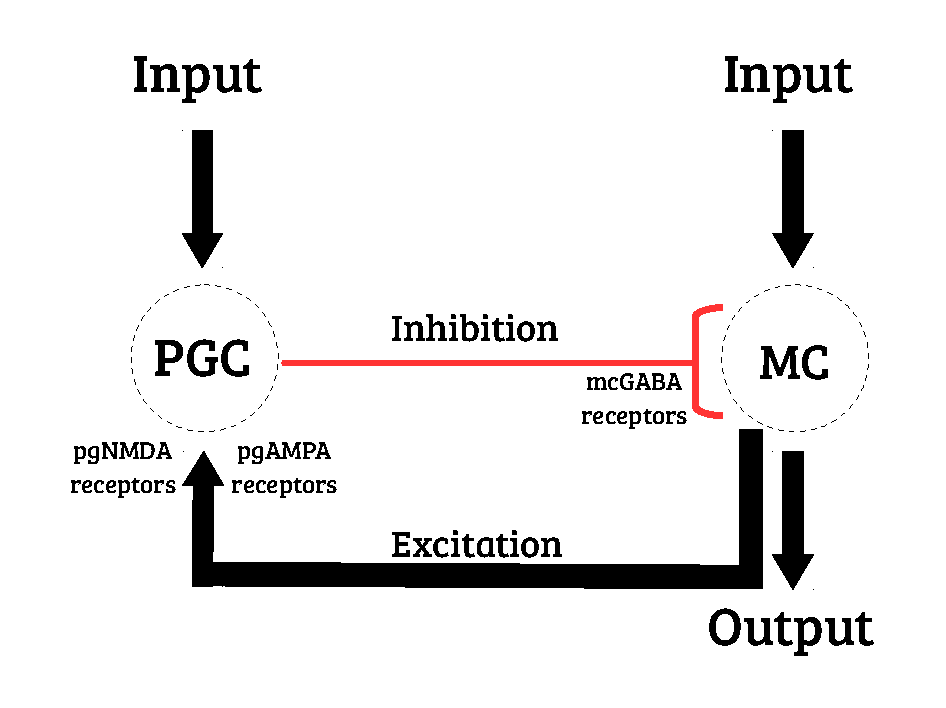
\includegraphics[scale=0.6]{images/Circuit_Diagram}
\end{figure}
\begin{itemize}
\item Used a model of the OB (modified from $[4]$).
\item Modeled MC - PGC (mitral cells - periglomerular cells), focusing on recurrent and feed - forward inhibition in the glomerular layer.
\end{itemize}
\end{block}

\begin{block}{Method}
 
\begin{figure}
\center
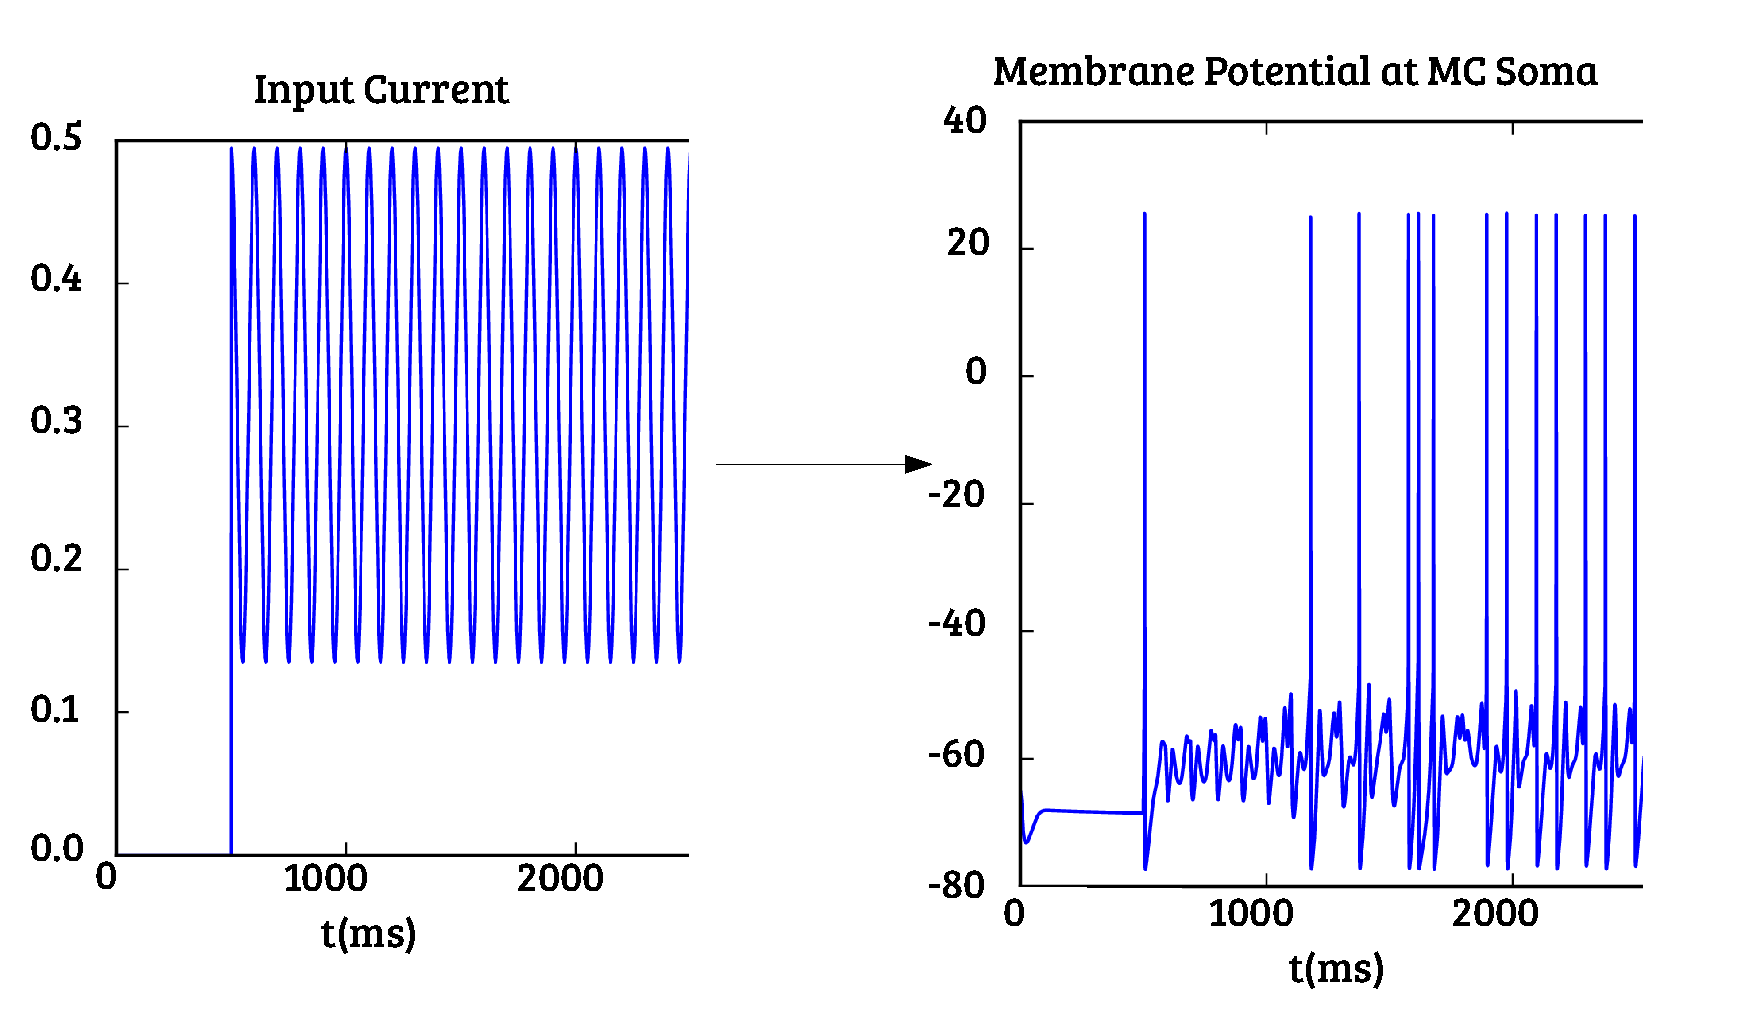
\includegraphics[scale=1.2]{images/Figure2}
\end{figure}
\begin{itemize}
\item Used sinusoidal currents of varying frequencies as input, using the equation:
\begin{equation}
y(t) = csin(2 \pi ft + \varphi) + 0.18. 
\end{equation}
\item phase $(\varphi) = 0$ and strength of input to MC $(c) = 0.45nA$.
\item PGC input strength was adjusted by multiplying $0.45nA$ by the values: $0.2, 0.3, 0.4, 0.5$ and $0.6$.
\item MC - PGC excitation strength varied using $W_{exc}$ values: $2.0, 4.0, 6.0, 8.0$ and $10.0$.
\item PGC - MC inhibition strength varied using $W_{inh}$ values: $1.0, 2.0, 3.0, 4.0$ and $5.0$.
\item Frequency $(f)$ of input ranged between 1.0Hz and 40.0Hz (with step size 1.0).
\item Parameter combinations: PGC input strength, MC - PGC excitation strength and PGC - MC inhibition strength.
\end{itemize}
      	
\begin{itemize}
\item constructed frequency tuning curves
\item extracted the peakresonance frequency and the strength of the tuning $Q$, measured as:
\begin{equation}
Q = \frac{(F_{max} - F_{min})}{<F>}
\end{equation}
\item $F_{max}$ and $F_{min}$ is the maximum and minimum firing rate.
\item $<F>$ is the mean firing rate over all measured frequencies.
\end{itemize}
      	
\end{block}

\end{column}




    \begin{column}{.48\linewidth}
      \begin{block}{Results}
      	\begin{figure}
      		\center
      		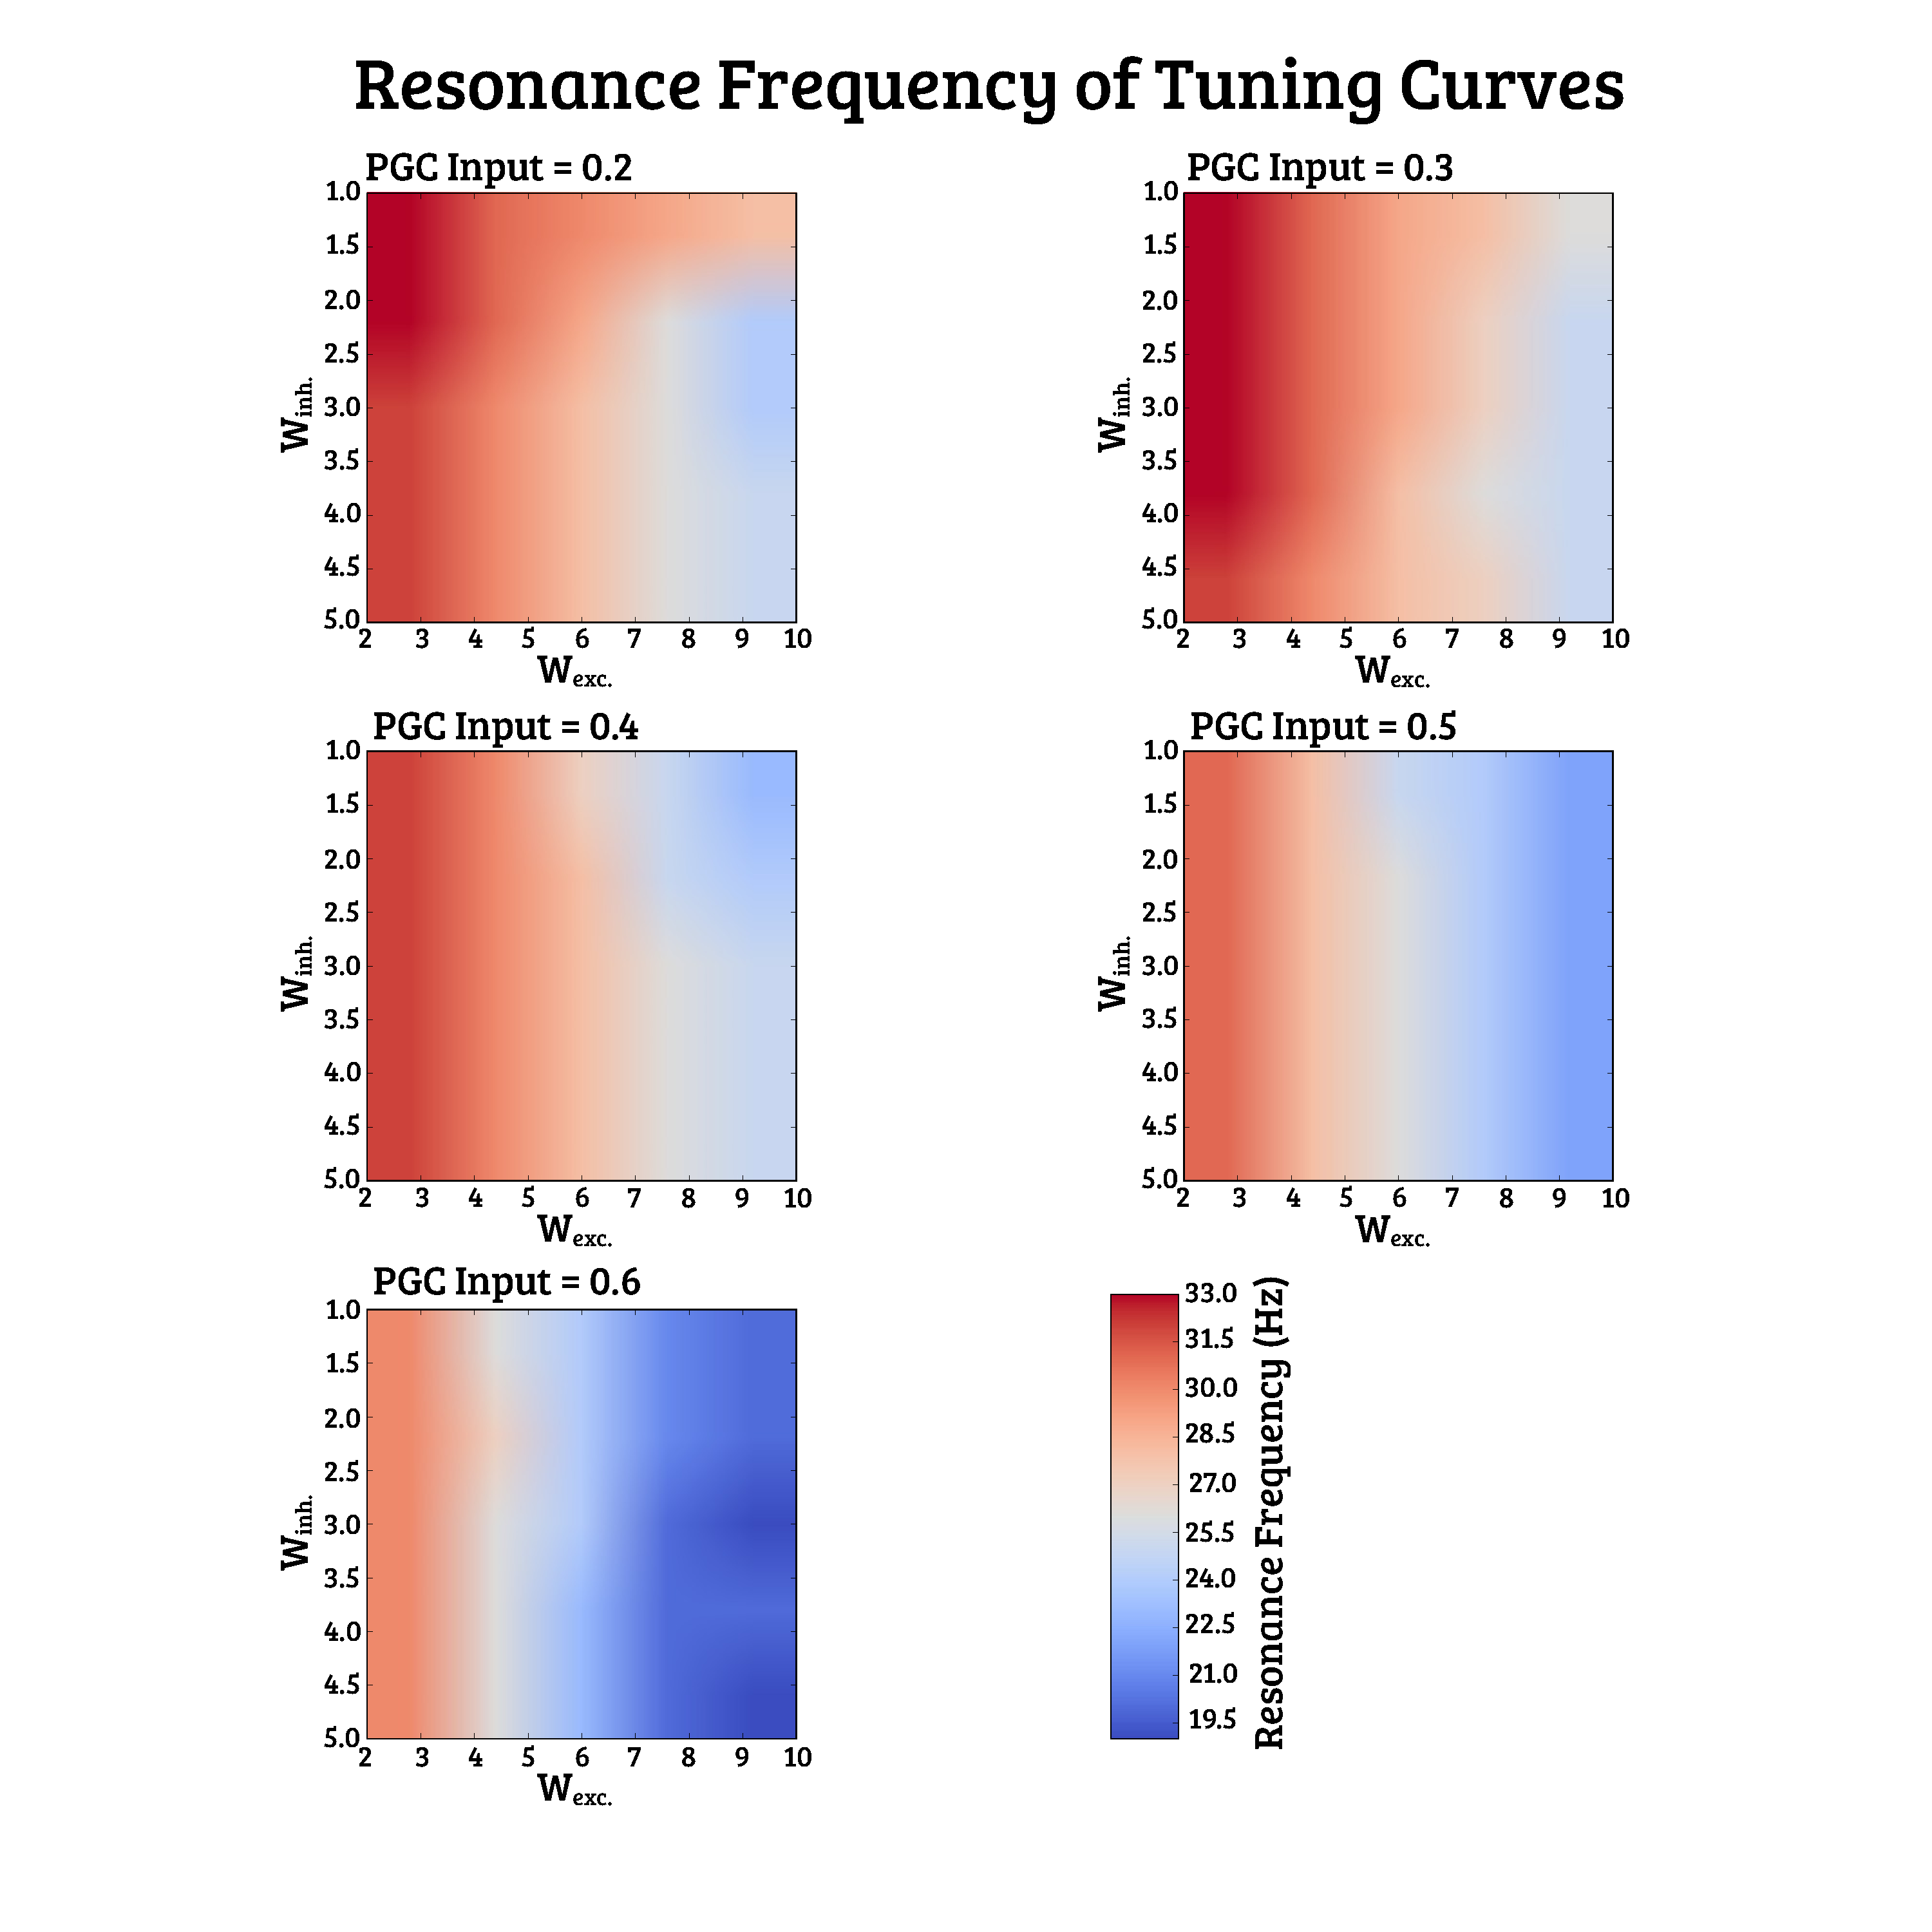
\includegraphics[scale=0.5]{images/Contour_plot_tuning_frequency}
      		\end{figure} 
        We found that the resonance frequency decreased as the excitation of the PGC (both from the input and from the MC) increased, whereas the strength of the PGC inhibition onto the MC did not seem to have a strong effect. 
        Furthermore, the resonance strength increased with the strength of the excitatory connection between the MC and the PGC when the PGC received sufficient external input from olfactory stimuli.
      \end{block}

      \begin{block}{Discussion}
      	\begin{figure}
      		\center
      		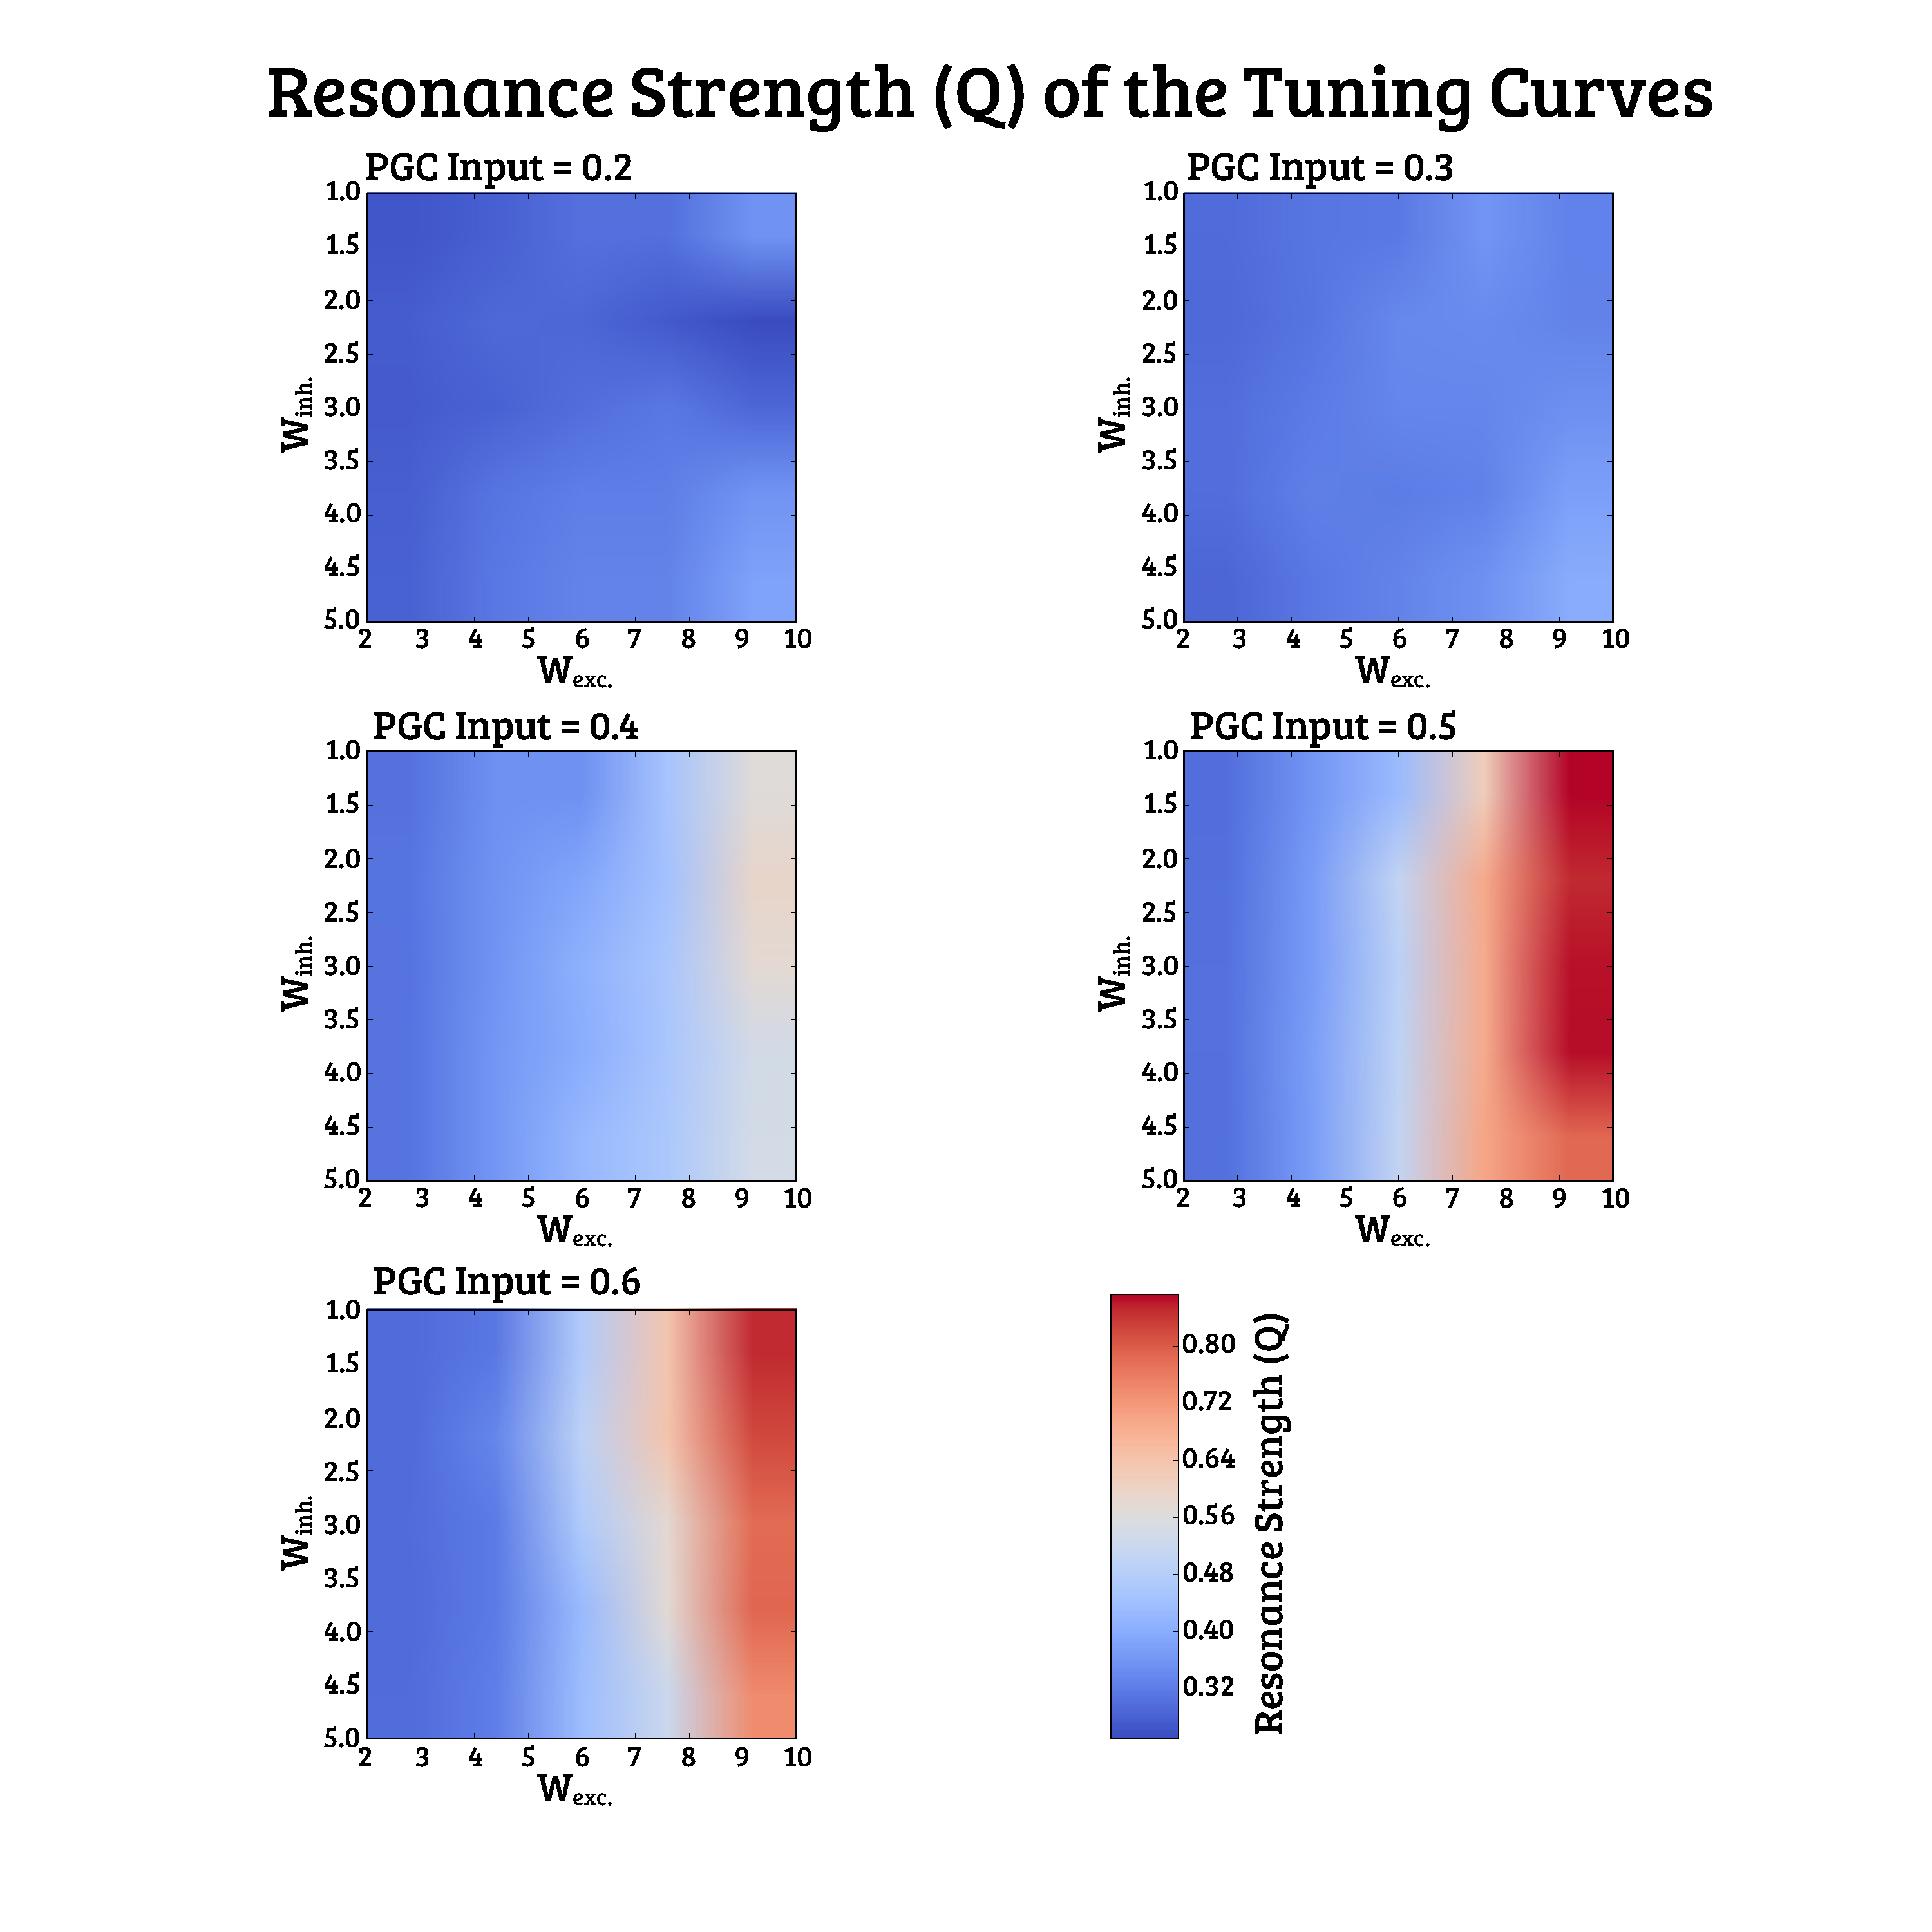
\includegraphics[scale=0.5]{images/Contour_plot_tuning_strength}
      		\end{figure} 
        These results suggest that the MC can indeed show frequency tuning and that this depends on the strength of the excitatory synaptic input to the PGC, which provide inhibitory input to the MC.
        However, the observed frequency tuning occurred in a narrow range ($19.5Hz – 33.0Hz$).
        Future work should investigate how the OB could use this frequency tuning to obtain information about the surrounding olfactory scene.
      \end{block}
    \end{column}
  \end{columns}
\end{frame}
\end{document}

%%%%%%%%%%%%%%%%%%%%%%%%%%%%%%%%%%%%%%%%%%%%%%%%%%%%%%%%%%%%%%%%%%%%%%%%%%%%%%%%%%%%%%%%%%%%%%%%%%%% 
%%% Local Variables: 
%%% mode: latex
%%% TeX-engine: xetex
%%% End: